%% =============================================================================
%% ОБЩИЕ ПРАВИЛА (для людей и для ИИ-агентов)
%% =============================================================================
%% 1. Это черновик ОДНОГО участника. Редактируй только этот файл.
%% 2. Не меняй чужие файлы в папке drafts/.
%% 3. Не трогай корневой main.tex, преамбулу, стили (.cls, .sty), .github/.
%% 4. Можно использовать существующие метки (\ref, \label, \cite), но не переименовывай их без согласования.
%% 5. Новые рисунки складывай в figures/ с уникальным именем: <имя>_<смысл>.png.
%% 6. Новые источники (BibTeX) пришли Давиду (david_final.tex) или в issues.
%% 7. Сохраняй статью в формате IEEEtran; не меняй шрифты/поля.
%% 8. После правки скинь файл координатору; сборка PDF делается в main.tex.
%% =============================================================================

%% УЧАСТНИК: Дима (@DmitryRekun)
%% РАЗДЕЛЫ: Neurocontrol + Neuro-symbolic control + Examples (Kaspersky MLAD, Amazon, Unitree G1)
%%
%% ЧТО СДЕЛАНО В ЭТОЙ РЕДАКЦИИ:
%%   - Neurocontrol переписан с опорой на обзоры 2024-2025 (Lawrence2024, Park2025rl).
%%   - Пример с "яблоком" заменён на промышленный пример (пастеризационная установка).
%%   - Схема классификации нейроуправления перерисована (диаграмма Венна из трёх
%%     свойств: approximation / optimization / adaptation) + добавлена таблица
%%     tab:neurocontrol_schemes с привязкой каждой схемы к установке.
%%   - Рисунок fig:pid_controller перенесён в раздел Neurocontrol (он показывает
%%     именно схему с самонастройкой) и получил корректную подпись; МЕТКА НЕ
%%     ПЕРЕИМЕНОВАНА.
%%   - Шесть детекторов Kaspersky MLAD свёрнуты из шести абзацев в таблицу
%%     tab:mlad_detectors; добавлены технические факты из Kaspersky ICS CERT.
%%   - Amazon: убрана публицистика про ChatGPT, добавлены проверяемые факты
%%     (Automated Reasoning checks GA 08.2025, Vulcan, Automated Reasoning CFP).
%%   - Unitree G1: сокращено, добавлены реальные характеристики платформы и
%%     ссылка на работу по нейро-символическому планированию 2025.
%%   - Добавлен связующий абзац, соединяющий три примера с разрабатываемым
%%     контроллером пастеризационной установки.
%%
%% !!! ДАВИДУ: в тексте появились НОВЫЕ ключи \cite. Готовые BibTeX-записи для
%% !!! bib/links.bib лежат В КОНЦЕ ЭТОГО ФАЙЛА (закомментированный блок).
%% !!! Пока они не добавлены в bib/links.bib, в PDF на их месте будет [?].
%% !!! Новые ключи: Lawrence2024, Park2025rl, Zribi2025, Bhuyan2024,
%% !!! Colelough2025, Confalonieri2025, KasperskyICS, AWS2025ar,
%% !!! AmazonVulcan2025, AmazonAR2025, UnitreeG1, Attolino2025.
%% =============================================================================

\section{Neurocontrol}

Neurocontrol denotes the use of trainable neural approximators as components of
a feedback loop. The field separated from general neural network research at the
end of the 1980s, although its premise is older. Cybernetics describes
regulation in machines and in living organisms by the same formal means, and
neurocontrol inherits from this view two properties: a control system that
improves its own behaviour during operation, and parallel rather than sequential
processing of sensor data~\cite{Uskov_2004, Neurocomputers}. Recent surveys of
machine learning in the process industries treat these properties as the
practical reason for adopting learned components, because such components absorb
plant behaviour that first-principles models describe
poorly~\cite{Lawrence2024}.

A pasteurization unit exhibits exactly this class of behaviour. Heat transfer in
the plate heat exchanger is nonlinear, the holding tube introduces a transport
delay that depends on the flow rate, and fouling gradually reduces the gain of
the heating loop over a production run. A proportional--integral--derivative
(PID) controller tuned for a clean exchanger and a nominal flow therefore
detunes as the shift proceeds. A learned component restores performance by
following the changed plant instead of waiting for a manual
retune~\cite{Park2025rl}.

Early neurocontrol was driven by a stronger ambition: a universal regulator that
looks like a black box from the outside. Such a regulator would be wired to
sensors, actuators, neighbouring controllers, and an efficiency module that
scores its behaviour against a chosen criterion. The operator would declare only
the target state, and the trained controller would find its own path to that
state and keep correcting itself from the plant response. The ambition remains
attractive, yet it is unacceptable in food processing, where the holding
temperature has to be demonstrably maintained and every intervention has to be
traceable. Current work on learning-based control accordingly shifts the
emphasis from unconstrained learning towards learned components with stated
stability and safety properties~\cite{Lawrence2024, Park2025rl}.

Neural network methods for control problems are classified by the capability
that the network supplies to the loop. Approximation replaces a mapping that is
hard to derive analytically, optimization improves a performance index over a
horizon, and adaptation keeps an existing regulator matched to a drifting plant.
Fig.~\ref{fig:neuro_control_classification} places the five schemes used in
practice within these three capabilities, and
Table~\ref{tab:neurocontrol_schemes} states what the network learns in each
scheme and how the scheme applies to the pasteurization unit.

\begin{figure}[ht]
  \centering
  \begin{adjustbox}{width=\columnwidth}
    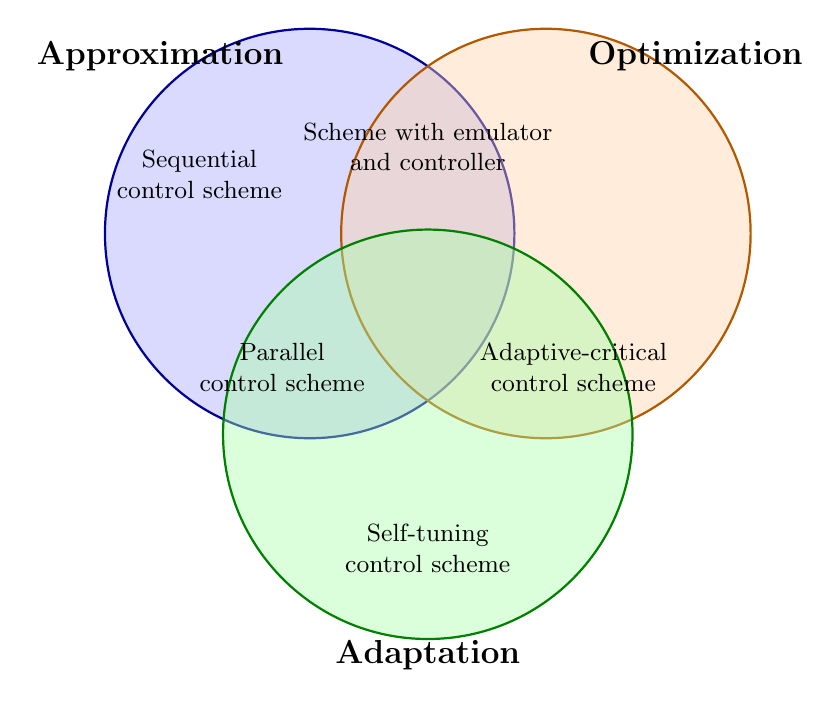
\begin{tikzpicture}[
        capability/.style={circle, minimum size=52mm, draw, thick,
          fill opacity=0.42, text opacity=1},
        scheme/.style={align=center, font=\small, inner sep=1pt},
        capname/.style={align=center, font=\bfseries\large}
      ]

      \node[capability, draw=blue!60!black,   fill=blue!35]   at (-1.5, 0.85) {};
      \node[capability, draw=orange!70!black, fill=orange!35] at ( 1.5, 0.85) {};
      \node[capability, draw=green!50!black,  fill=green!35]  at ( 0.0,-1.70) {};

      \node[capname] at (-3.4, 3.1) {Approximation};
      \node[capname] at ( 3.4, 3.1) {Optimization};
      \node[capname] at ( 0.0,-4.5) {Adaptation};

      \node[scheme] at (-2.90, 1.60) {Sequential\\ control scheme};
      \node[scheme] at ( 0.00, 1.95) {Scheme with emulator\\ and controller};
      \node[scheme] at (-1.85,-0.85) {Parallel\\ control scheme};
      \node[scheme] at ( 1.85,-0.85) {Adaptive-critical\\ control scheme};
      \node[scheme] at ( 0.00,-3.15) {Self-tuning\\ control scheme};

    \end{tikzpicture}
  \end{adjustbox}

  \caption{Classification of neural network methods for solving control
  problems}
  \label{fig:neuro_control_classification}
\end{figure}

\begin{table}[ht]
  \caption{Neurocontrol schemes and their role on the pasteurization unit}
  \label{tab:neurocontrol_schemes}
  \centering
  \footnotesize
  \setlength{\tabcolsep}{3pt}
  \renewcommand{\arraystretch}{1.2}
  \begin{tabular}{p{1.75cm}p{2.55cm}p{3.45cm}}
    \hline
    \textbf{Scheme} & \textbf{What the network learns} & \textbf{Role on the
    unit} \\
    \hline
    Sequential & The inverse model of the plant, used directly as a regulator &
    Removes the need for an analytical model of the heating section, but demands
    a data set that covers all operating modes \\
    Scheme with emulator and controller & A model of the plant, through which
    the second network is trained & Allows offline training on a simulated
    exchanger before the controller touches the real unit \\
    Parallel & A corrective signal added to the output of a conventional
    regulator & Compensates the residual error of the existing PID loop without
    replacing it \\
    Adaptive-critical & An estimate of the future cost and a policy that
    minimizes it & Suitable for coordinating heating, holding, and cooling
    stages over a horizon rather than pointwise \\
    Self-tuning & The dependence of the regulator coefficients on the current
    plant state & Keeps the PID loop matched to fouling and to changes of flow
    rate; used in this work \\
    \hline
  \end{tabular}
\end{table}

The self-tuning scheme is the least invasive of the five, because the
conventional regulator stays in the loop and the network only moves its
coefficients. Fig.~\ref{fig:pid_controller} shows this scheme for the
pasteurization unit: delayed samples of the pasteurization temperature and of
the opening of the steam valve are mapped to the proportional, integral, and
derivative coefficients of the PID controller. Reinforcement learning is now
used to adjust such a mapping online, which removes the fixed learning rate that
limited earlier neural tuners~\cite{Zribi2025}. This scheme is therefore taken
as the basis of the controller described below.

\begin{figure}[ht]
  \centering
  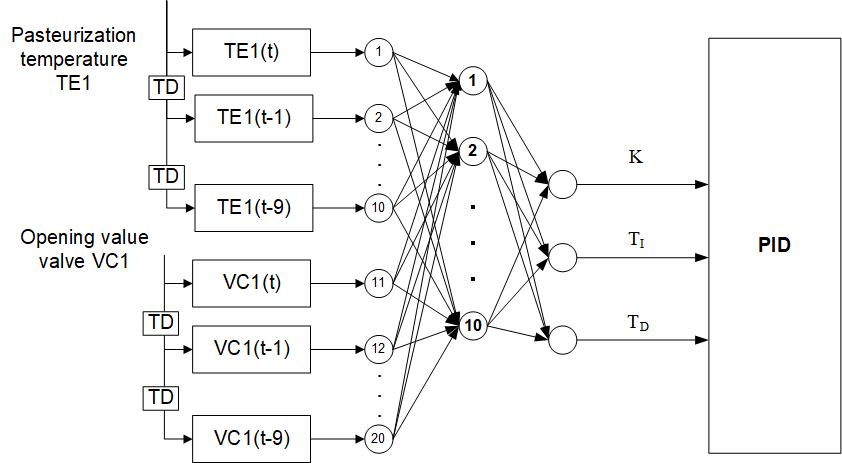
\includegraphics[width=\columnwidth]{figures/Neuro-adjuster-PID.png}
  \caption{Neural tuner of the PID controller of the pasteurization unit}
  \label{fig:pid_controller}
\end{figure}

None of the five schemes, however, states why a correction was applied. The
network reports what to do, not on what grounds. Closing this gap requires
knowledge that is represented explicitly, which is the subject of the next
section.

\section{Neuro-symbolic control}

Neuro-symbolic AI combines the two historical paradigms of the field. Symbolic
AI represents a task as structures of signs and derives conclusions by logical
inference. Statistical AI, and neural networks in particular, extracts
regularities from data and solves recognition tasks that resist formalization.
The two were long treated as competitors, and the symbolic branch was widely
declared obsolete~\cite{Bhuyan2024}.

Systematic reviews of the last two years show that the combination has become a
research field in its own right rather than a compromise between the
paradigms~\cite{Colelough2025}. A symbolic layer supplies the constraints,
definitions, and causal relations that a network would otherwise have to infer
from data. Consequently, a hybrid system reaches comparable accuracy on a
smaller training set, and its conclusions can be traced back to explicit
statements. Ontologies act as the interface between the layers, because they fix
the vocabulary in which a numerical output becomes an assertion about the
plant~\cite{Confalonieri2025}.

The value of the combination is clearest when a prediction has to become an
action on a particular piece of equipment. A network trained on pasteurizer
telemetry can report that the temperature at the outlet of the holding tube will
fall below the pasteurization setpoint within the next minute. Taken alone, this
number identifies neither the cause nor the admissible response. A symbolic
layer that holds the ISA-88 model of the unit and the ISA-5.1 documentation of
its loops resolves which control module is affected, checks whether the running
phase permits a setpoint change, and reports the chain of assertions that led to
the recommendation~\cite{ISA-88-formalization, isa-5.1-ostis}. The operator thus
receives a conclusion together with its justification.

OSTIS Technology provides such a layer in a form suitable for a controller.
Standards, plant structure, and process knowledge reside in a single semantic
network, so a neural module and a rule set operate on the same representation
instead of on separate copies~\cite{Golenkov2019, ivaniuk2025neurosymbolic}.
Earlier work on the same unit showed that neural modules attach to an OSTIS
knowledge base without a dedicated integration format, which keeps the symbolic
layer authoritative and the neural layer
replaceable~\cite{Golovko2018integration, ivaniuk2024neurosemantic}.

\section{Examples}

Three deployments show the range of the approach at different scales: anomaly
detection over industrial telemetry, verified reasoning in enterprise software
and warehouse robotics, and layered control of a general-purpose robot.

\subsection{Kaspersky MLAD}

Kaspersky MLAD observes the telemetry of a technological process and reports
deviations from its predicted behaviour~\cite{KasperskyMLAD}. For this system an
anomaly is a statistically significant divergence between measured and forecast
values, not a violation of a fixed threshold. The purpose is to expose the early
signs of a failure long before they affect production.
Fig.~\ref{fig:MLAD} shows the position of the system in the production loop.

\begin{figure*}[ht]
    \centering
    \thispagestyle{empty}
    % ограничиваем ширину и высоту, сохраняем пропорции
    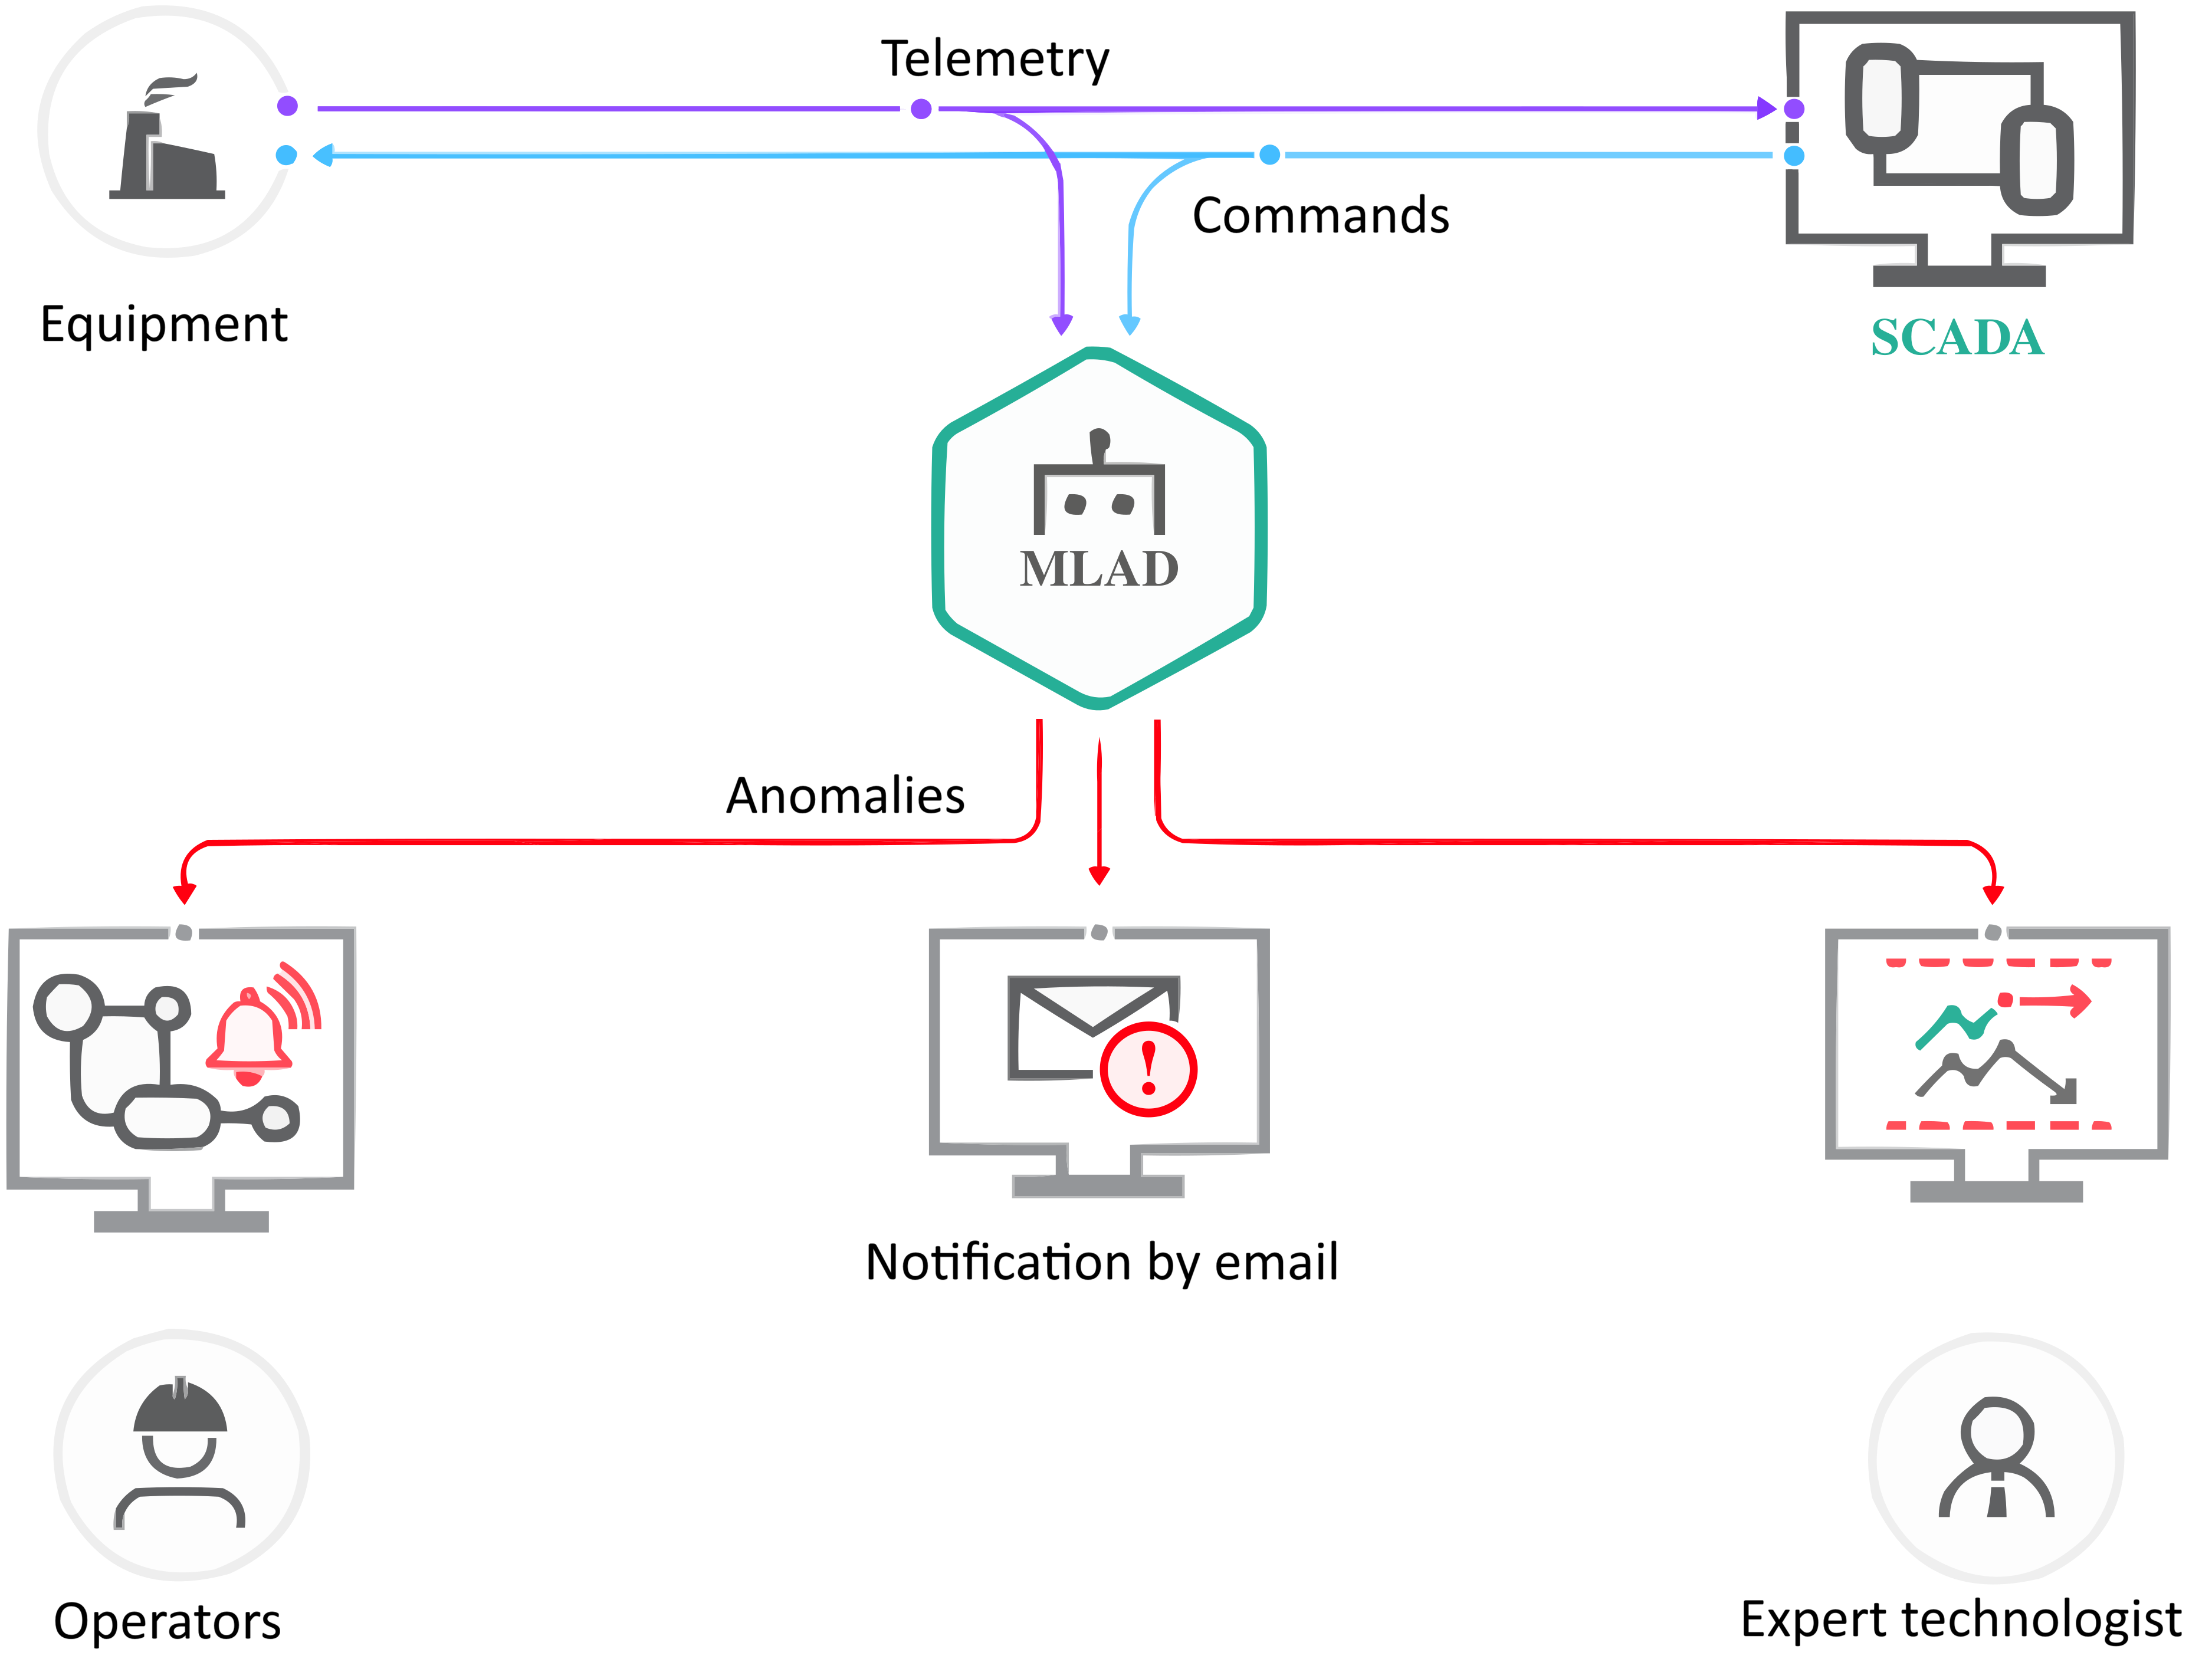
\includegraphics[width=\linewidth, height=0.9\textheight, keepaspectratio]
        {figures/MLAD_in_industry.png}
    \caption{Kaspersky MLAD system in the production process}
    \label{fig:MLAD}
\end{figure*}

The system was developed because conventional monitoring reacted to events that
had already occurred and did not scale to the available data. A single facility
produces tens of thousands of tags updated roughly 10 times per second, with
years of history behind them~\cite{KasperskyICS}.

MLAD does not intervene in the process. It modifies neither the control logic
nor the transmission of data, and the final decision remains with the operator.
This property is essential for a pasteurization unit, where a monitoring system
must not become an uncontrolled participant in the control loop.

Technically the system treats telemetry as a multivariate time series and trains
a recurrent network with long short-term memory cells to reproduce its normal
behaviour~\cite{KasperskyICS}. Because process variables are mutually dependent,
the learned relations between tags carry most of the diagnostic information.
Convolutional, densely connected, and temporal convolutional architectures serve
the accompanying classification and preprocessing tasks. MLAD is therefore a set
of interacting neural modules rather than a single model.

Six analytical processors work on top of this forecast.
Table~\ref{tab:mlad_detectors} summarizes their functions.

\begin{table}[ht]
  \caption{Analytical processors of Kaspersky MLAD}
  \label{tab:mlad_detectors}
  \centering
  \footnotesize
  \setlength{\tabcolsep}{3pt}
  \renewcommand{\arraystretch}{1.2}
  \begin{tabular}{p{2.35cm}p{5.45cm}}
    \hline
    \textbf{Processor} & \textbf{Function} \\
    \hline
    Predictive detector & Forecasts the current values of the process variables
    and reports a significant divergence from the observed ones; trained on
    history without expert labels, so previously unknown anomalies are also
    detected \\
    State classifier & Separates operating modes with an elliptic envelope built
    from Gaussian models and reports states that match no known mode \\
    Rule-based diagnostic detector & Checks symptoms known in advance:
    persistent threshold excess, monotone drift over a period, step changes, and
    values frozen at one level \\
    Time-to-threshold detector & Estimates the time remaining until a variable
    reaches a given threshold and triggers when this time falls below the
    configured margin \\
    Stream processor & Resamples incoming telemetry to a uniform time grid and
    repairs stream defects such as gaps, invalid values, and late observations
    \\
    Event processor & Analyses sequences of discrete events and reports unusual
    sequences, including combinations of operator actions and earlier alarms \\
    \hline
  \end{tabular}
\end{table}

\begin{figure*}[ht]
    \centering
    \thispagestyle{empty}
    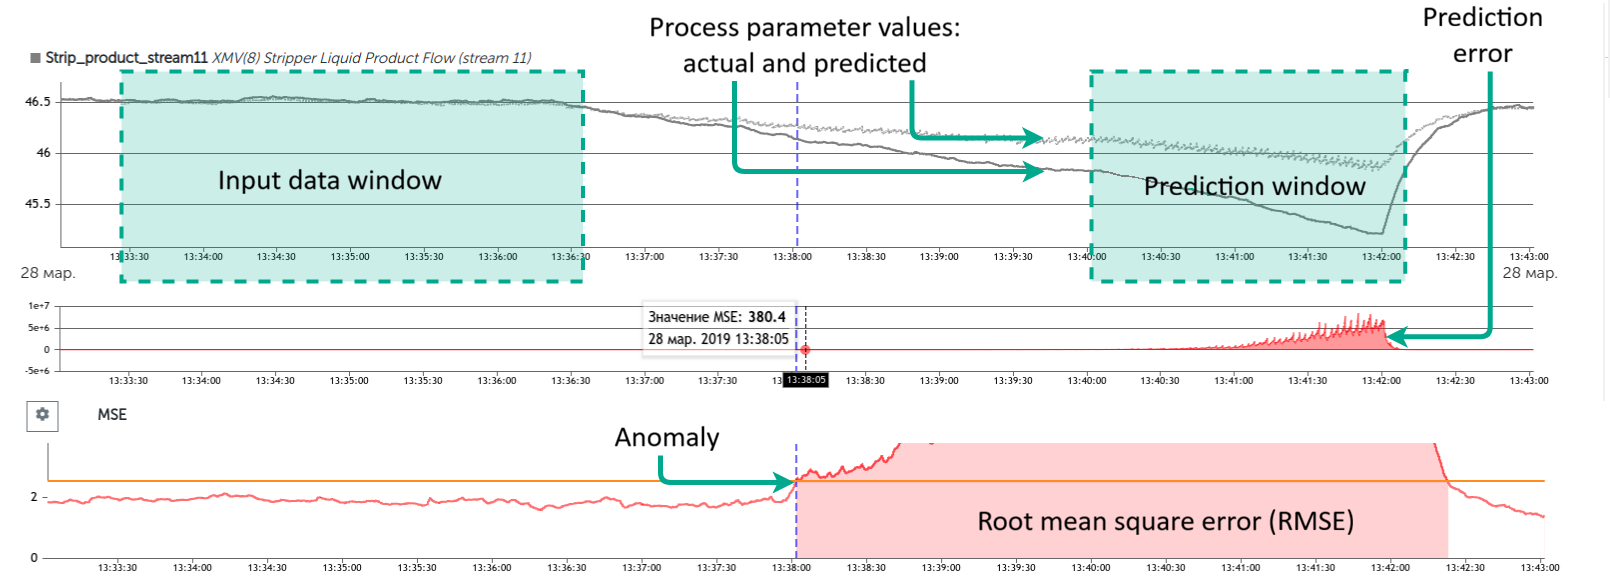
\includegraphics[width=\linewidth]{figures/MLAD_example.png}
    \caption{Example of the operation of the Kaspersky MLAD predictive detector}
    \label{fig:MLADex}
\end{figure*}

The predictive detector deserves separate attention, because it defines the
behaviour of the whole product. It forms an input window from the arriving
process data and produces a prediction window that describes the near future of
the object. The individual prediction errors are then weighted and reduced to a
mean squared error. A second model compares this error with a threshold learned
during training and decides whether an anomaly has occurred.
Fig.~\ref{fig:MLADex} shows the sequence on real data.

MLAD illustrates both the strength and the limit of a purely statistical
detector. It finds deviations that no expert described in advance, yet it
reports them in terms of tags and error magnitudes. Turning such a report into a
statement about a specific control module still requires an explicit model of
the unit.

\subsection{Amazon}

Amazon applies the neuro-symbolic combination in the opposite direction: formal
reasoning constrains the output of a neural model rather than the other way
round. The motivation is the one that drives the whole field, namely that a
statistical model produces a plausible answer but cannot certify
it~\cite{Marcus2024, WSJ2024}.

Automated Reasoning checks became generally available in Amazon Bedrock
Guardrails in August 2025. The service converts a body of domain documents into
a logical policy and then verifies model answers against that policy by formal
methods instead of by a second neural model. Amazon reports verification
accuracy up to 99\% and builds a policy from documents of up to 122,880 tokens
in a single pass~\cite{AWS2025ar}.

The same separation of roles is applied to physical systems. The Vulcan
manipulator, presented in 2025, complements visual perception with force
feedback and handles about 75\% of the items stored in a fulfilment
centre~\cite{AmazonVulcan2025}. Reliability there comes from constraints that
hold regardless of what the learned policy proposes. Amazon also funds external
work on the same problem: the Automated Reasoning call for proposals of autumn
2025 is directed at sound neuro-symbolic reasoning that couples language models
with automated solvers and proof checking~\cite{AmazonAR2025}.

The lesson for industrial control is the division of responsibility. The learned
component proposes an action, the formal component admits or rejects it, and a
rejection is explainable by construction.

\subsection{Humanoid robot Unitree G1 (China)}

Humanoid platforms show the layered organization of a hybrid controller at full
scale. Unitree G1 is a research platform with 23 to 43 degrees of freedom,
equipped with a three-dimensional lidar and a depth camera and supplied with an
open software development kit, ROS~2 support, and a unified robot
model~\cite{UnitreeG1}. Low-level motion control alone does not make such a
platform useful in an unstructured environment. The robot has to interpret
context, plan a sequence of actions, and revise the plan when the environment
contradicts it.

Neither paradigm covers this task alone. A learned policy generalizes poorly to
situations absent from its training data, whereas a symbolic planner fails on
noisy perception. A hybrid architecture for such a robot is therefore organized
in four layers:

\begin{enumerate}
    \item \textbf{Perception.} Deep networks process camera, lidar, and tactile
    data, and produce object detections, poses, and gestures.
    \item \textbf{Symbolic model.} Domain ontologies and a logic programming
    language hold statements about the world, such as the position of an object
    or the state of a door, and support consistency checks and causal chains.
    \item \textbf{Interface.} A translator converts continuous network outputs
    into discrete assertions and symbolic plans into target trajectories for the
    low-level controllers.
    \item \textbf{Planner.} A classical planner combined with reinforcement
    learning produces an action sequence that respects both the physical
    constraints of the robot and the logical conditions of the task.
\end{enumerate}

Unitree has not announced neuro-symbolic control as a product feature, so this
architecture describes what the platform admits rather than what it ships. The
research direction is nevertheless active. Recent work performs symbolic
planning with a locally hosted language model of about 1.5 billion parameters
and reports 70.6\% plan validity across several domains, which brings hybrid
planning within reach of an on-board computer~\cite{Attolino2025}.

The three examples differ in scale but share one structure. A neural component
handles the continuous and noisy part of the task, an explicit model handles the
part that has to be justified, and an interface converts one into the other. The
controller described in the following sections applies this structure to a
pasteurization unit, with OSTIS Technology in the role of the explicit model.

%% =============================================================================
%% НОВЫЕ ИСТОЧНИКИ ДЛЯ bib/links.bib — ДЛЯ ДАВИДА (@Bidway)
%% Скопировать блок ниже в bib/links.bib БЕЗ символов "%% " в начале строк.
%% Формат согласован с существующими записями. Ключи уже используются в тексте
%% выше, поэтому до добавления записей в PDF будет [?].
%% =============================================================================
%%
%% @article{Lawrence2024,
%%   author  = {Lawrence, Nathan P. and Damarla, Seshu Kumar and Kim, Jong Woo
%%              and Tulsyan, Aditya and Amjad, Faraz and Wang, Kai and Chachuat,
%%              Benoit and Lee, Jong Min and Huang, Biao and Gopaluni, R.
%%              Bhushan},
%%   title   = {Machine learning for industrial sensing and control: A survey
%%              and practical perspective},
%%   journal = {Control Engineering Practice},
%%   volume  = {145},
%%   pages   = {105841},
%%   year    = {2024},
%%   doi     = {10.1016/j.conengprac.2024.105841}
%% }
%%
%% @article{Park2025rl,
%%   author  = {Park, Joonsoo and Jung, Hyein and Kim, Jong Woo and Lee, Jong
%%              Min},
%%   title   = {Reinforcement Learning for Process Control: Review and Benchmark
%%              Problems},
%%   journal = {International Journal of Control, Automation and Systems},
%%   volume  = {23},
%%   number  = {1},
%%   pages   = {1--40},
%%   year    = {2025},
%%   doi     = {10.1007/s12555-024-0990-1}
%% }
%%
%% @article{Zribi2025,
%%   author  = {Zribi, Ali and Taouil, Hajer},
%%   title   = {Adaptive reinforcement learning-based tuning of neural {PID}
%%              controllers for nonlinear systems},
%%   journal = {Journal of Vibration and Control},
%%   year    = {2025},
%%   doi     = {10.1177/10775463251404852}
%% }
%%
%% @article{Bhuyan2024,
%%   author  = {Bhuyan, Bikram Pratim and Ramdane-Cherif, Amar and Tomar, Ravi
%%              and Singh, T. P.},
%%   title   = {Neuro-symbolic artificial intelligence: a survey},
%%   journal = {Neural Computing and Applications},
%%   volume  = {36},
%%   number  = {21},
%%   pages   = {12809--12844},
%%   year    = {2024},
%%   doi     = {10.1007/s00521-024-09960-z}
%% }
%%
%% @misc{Colelough2025,
%%   author       = {Colelough, Brandon C. and Regli, William},
%%   title        = {Neuro-Symbolic {AI} in 2024: A Systematic Review},
%%   howpublished = {\url{https://arxiv.org/abs/2501.05435}},
%%   year         = {2025},
%%   note         = {arXiv:2501.05435. Accessed: 2026-09-03}
%% }
%%
%% @article{Confalonieri2025,
%%   author  = {Confalonieri, Roberto and Guizzardi, Giancarlo},
%%   title   = {On the multiple roles of ontologies in explanations for
%%              neuro-symbolic {AI}},
%%   journal = {Neurosymbolic Artificial Intelligence},
%%   year    = {2025},
%%   doi     = {10.3233/NAI-240754}
%% }
%%
%% @misc{KasperskyICS,
%%   author       = {{Kaspersky ICS CERT}},
%%   title        = {{MLAD}: Machine Learning for Anomaly Detection},
%%   howpublished = {\url{https://ics-cert.kaspersky.com/publications/mlad-machine-learning-for-anomaly-detection/}},
%%   year         = {2025},
%%   note         = {Accessed: 2026-09-03}
%% }
%%
%% @misc{AWS2025ar,
%%   author       = {{Amazon Web Services}},
%%   title        = {Minimize {AI} hallucinations and deliver up to 99\%
%%                   verification accuracy with Automated Reasoning checks},
%%   howpublished = {\url{https://aws.amazon.com/blogs/aws/minimize-ai-hallucinations-and-deliver-up-to-99-verification-accuracy-with-automated-reasoning-checks-now-available/}},
%%   year         = {2025},
%%   note         = {Accessed: 2026-09-03}
%% }
%%
%% @misc{AmazonVulcan2025,
%%   author       = {{Amazon}},
%%   title        = {Introducing {Vulcan}: {Amazon's} first robot with a sense of
%%                   touch},
%%   howpublished = {\url{https://www.aboutamazon.com/news/operations/amazon-vulcan-robot-pick-stow-touch}},
%%   year         = {2025},
%%   note         = {Accessed: 2026-09-03}
%% }
%%
%% @misc{AmazonAR2025,
%%   author       = {{Amazon Science}},
%%   title        = {Automated Reasoning call for proposals --- Fall 2025},
%%   howpublished = {\url{https://www.amazon.science/research-awards/call-for-proposals/automated-reasoning-call-for-proposals-fall-2025}},
%%   year         = {2025},
%%   note         = {Accessed: 2026-09-03}
%% }
%%
%% @misc{UnitreeG1,
%%   author       = {{Unitree Robotics}},
%%   title        = {Humanoid robot {G1}},
%%   howpublished = {\url{https://www.unitree.com/g1/}},
%%   year         = {2025},
%%   note         = {Accessed: 2026-09-03}
%% }
%%
%% @misc{Attolino2025,
%%   author       = {Attolino, Nicholas and Capitanelli, Alessio and
%%                   Mastrogiovanni, Fulvio},
%%   title        = {Achieving Scalable Robot Autonomy via Neurosymbolic Planning
%%                   Using Lightweight Local {LLM}},
%%   howpublished = {\url{https://arxiv.org/abs/2505.08492}},
%%   year         = {2025},
%%   note         = {arXiv:2505.08492. Accessed: 2026-09-03}
%% }
%% =============================================================================
